\chapter{Modelling the interactions}
\label{ch:MC}

For any measurement in particle physics, a set of MC samples has to be generated in order to compare the experimental data to theoretical models.  These models include well known decay processes such as \ttbar{} production in the \SM{}, through to a multitude of theoretical predications. 
% WHICH ONES? DM, SUSY, ETC
% The following sections describe in more detail the generators and showerers used in this analysis
Any interaction can be modelled as a combination of discrete steps.
Firstly, the hard scattering process is generated at \LO{}, or if possible \NLO{}, to form short lived resonances which decay into the final state.
Additional parton interactions can be included at \LO{} and soft radiation included in the inital and final states.
All partons are then hadronised into colourless states and decayed (\textit{parton shower}), with the proton remnants forming the underlying event.
Finally, the interaction can be smeared depending on the effects of the detector being used.
Figure\,\ref{fig:GenEvent} shows diagrammatically an example simulated collision, where the hard scattering process is shown in red, the soft radiative processes in blue, the additional parton interactions in purple, the hadronisation in light green and parton shower in dark green.
\begin{figure}[htpb]
	\centering
	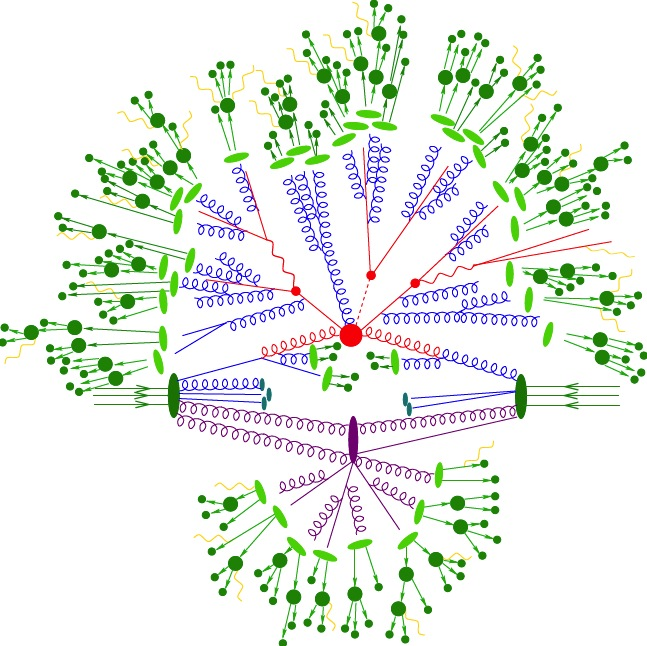
\includegraphics[width=\textwidth]{Figures/Generator_Event}
	\caption[ ]{  Figure taken from\,\cite{Gen:Event}.}
	\label{fig:GenEvent}
\end{figure}

\section{Hard interaction} % (fold)
\label{sub:hard_interaction}
The hard scattering process describes the interaction of two partons in the collider and the subsequent final state. 
It is modelled though Eq\,\ref{eq:pdf}, with the \PDF{}s being taken from data convoluted with the partonic cross section.
The partonic cross section is calculated from the \textit{matrix-element} of the interaction, directly taken from the Feynman diagrams through the Feynman rules.
% section hard_interaction (end)

\section{Underlying event} % (fold)
\label{sub:underlying_event}
\begin{itemize}
	\item Soft processes
	\item MPI
\end{itemize}
% section underlying_event (end)


\section{Colour reconnection} % (fold)
\label{sub:colour_reconnection}
% section colour_reconnection (end)

\section{Hadronisation} % (fold)
\label{sub:hadronisation}

The hadronisation process first introduce in Section TODO, models the colourless particles produced from the final state partons.
One model used is the Bowler-Lund parameterisation.
This involves

Because of the self interactions between gluons the strong field between two quarks can be represented by a confined tube of dimension $1+1$, otherwise known as a string. 
As the quarks move apart the potential energy in the string increases linearly by 1\GeV{}\fminv{}.
At some point the colour field contains enough potential energy that it is favourable to pair-produce quarks, which form two new colourless particles, breaking the string.
This broken string model is known as the \textit{Lund string model} TODO REF and is represented in Fig.\,\ref{fig:Lund}.
\begin{figure}[htpb]
	\centering
	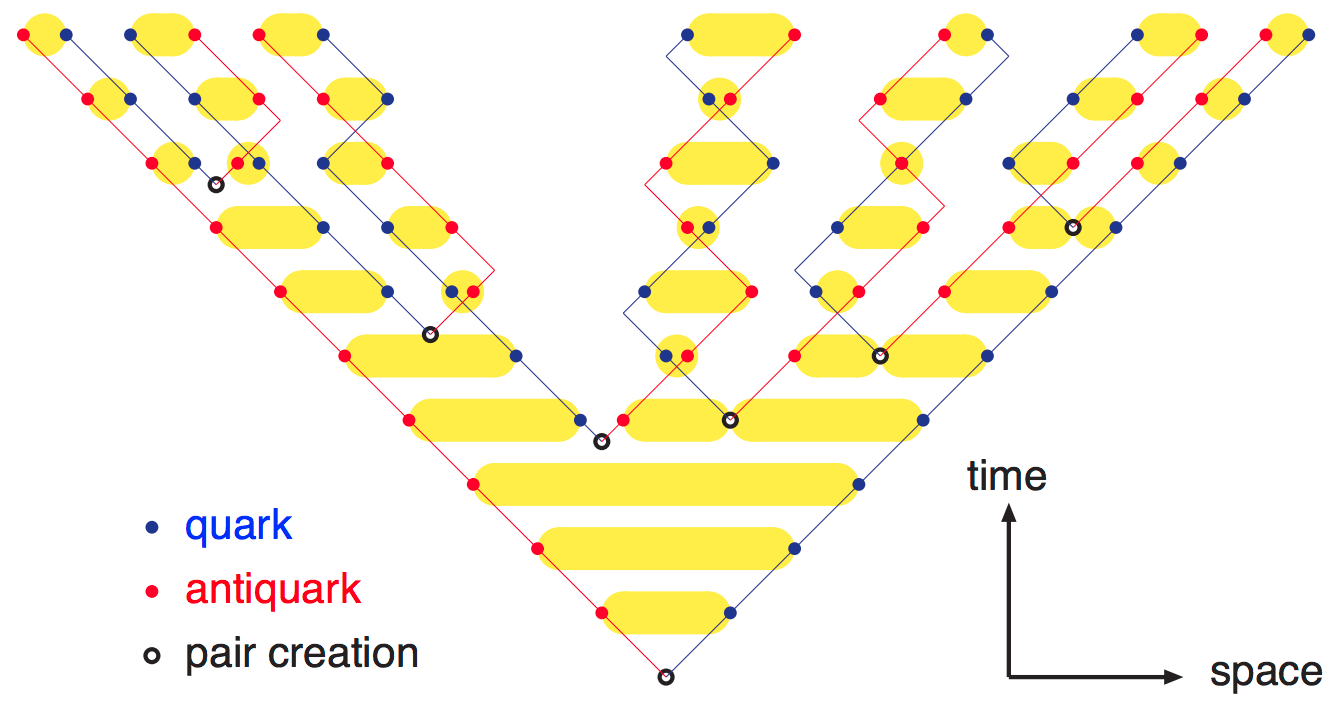
\includegraphics[width=0.8\textwidth]{Figures/Generator_Lund}
	\caption[ ]{ oscillation can be lorentz boosted, shown in rectangles. Figure taken from talk by Torbj\"orn Sj\"ostrand in \cite{Gen:Lund}.}
	\label{fig:Lund}
\end{figure}
As time evolves, if \qqbar{} pairs do not have enough potential in the colour field to pair-produce they end up oscillating around each other, forming the colourless mesons of the final state.
Additionally, \qqqbarqbar{} may be produced instead of \qqbar{} with the end result being the formation of baryons in the final state.

This approach is used in \pythia{}.
\begin{equation}
	\frac{dP}{d\pt} \propto \kappa (e^{\frac{\pi m_{\mathrm{T}}^2}{\kappa}})
\end{equation}
% section hadronisation (end)

\section{Parton shower} % (fold)
\label{sub:parton_shower}
TODO MOVE TO GENERATOR SECTION?
The final state particles, which can include additional partons that have been radiated from both the initial and final states (ISR and FSR), are represented by open lines.
As stated in Section\,\ref{sub:confinement}, these bare quarks rapidly hadronise, producing sprays of colourless particles.
% section parton_shower (end)




\section{Detector modelling} % (fold)
\label{sub:detector_modelling}

% section detector_modelling (end)


\section{\ttbar{} model generators}
\label{sec:ttMC}

\begin{itemize}
	\item Different parts of generator
	\item colour reconnection, matching, underlying event, etc
	\item models we use
	\item backgrounds?
\end{itemize}
\begin{table}
	\centering
		\caption{The set of simulated samples used in this thesis. They include four different signal \ttbar{} production samples and samples for the background production. The backgrounds are single top quark production, vector boson production in association with jets and multijet \QCD{}. }
		\label{tb:Gen}
		\resizebox{\linewidth}{!}{%
		\begin{tabular}{llllccc}
			 	& \textbf{Matrix}	& \textbf{Parton} & \textbf{Tune}	& \textbf{Cross section} 	  			& \textbf{Events}  	& \textbf{Luminosity} 	\\
			 	& \textbf{element}	& \textbf{shower} &  				& \textbf{(\pb{})} 	&  	\textbf{(\ten{6})}	& \textbf{(\fbinv{})} 	\\
			\multicolumn{7}{l}{\textbf{Models of \ttbar{} production}} \\
			\hline
			\vspace*{0.02cm}
			\powhegpythia{} & \powheg{} & \pythia{} & \CUET{}		& 831.76 & 154.9 & 186.3 \\ 
			\powhegherwig{} & \powheg{} & \herwig{} & \herwigtune{}	& 831.76 & 59.2  & 77.1 \\ 
			\mgamcLO{} 		& \mgamc{}	& \pythia{} & \CUETold{}  	& 831.76 & 10.1  & 12.2 \\ 
			\mgamcNLO{} 	& \mgamc{}	& \pythia{} & \CUETold{}  	& 831.76 & 30.4  & 36.6 \\ 

			\vspace*{0.02cm} \\
			\multicolumn{7}{l}{\textbf{Models of single top background production}} \\
			\hline
			\vspace*{0.02cm}
			Single top $t$-channel 			& \powheg{} 			& \pythia{} &	\CUETold{}  & 136.02	  & 66.9  & 492.0 \\ 
			Single anti-top $t$-channel	 	& \powheg{} 			& \pythia{} &	\CUETold{}  & 80.95	  	  & 38.8  & 479.4 \\ 
			Single top $tW$-channel 		& \powheg{} (v1)		& \pythia{} &	\CUETold{}  & 35.6		  & 7.9   & 223.2 \\ 
			Single anti-top $tW$-channel 	& \powheg{} (v1)		& \pythia{} &	\CUETold{}  & 35.6		  & 7.9   & 222.8 \\ 
			Single top/anti-top $s$-channel & \mgamc{} 				& \pythia{} &	\CUETold{}  & 6.35		  & 0.6    & 98.1 \\ 

			\vspace*{0.02cm} \\
			\multicolumn{7}{l}{\textbf{Models of vector boson background production}} \\
			\hline 
			\vspace*{0.01cm}
			Drell-Yan + 1 jet 			& \mgamc{}			& \pythia{} &	\CUETold{}	 & 	1016		  &  62.6  & 61.6 \\ 
			Drell-Yan + 2 jets  		& \mgamc{}			& \pythia{} &	\CUETold{}	 & 	331.4		  &  20.0  & 60.3 \\ 
			Drell-Yan + 3 jets  		& \mgamc{}			& \pythia{} &	\CUETold{}	 & 	96.36		  &  5.9   & 60.8 \\ 
			Drell-Yan + 4 jets  		& \mgamc{}			& \pythia{} &	\CUETold{}	 & 	51.4		  &  4.2   & 81.7 \\ 
			\Wboson{} boson + 1 jet 	& \mgamc{}			& \pythia{} &	\CUETold{}	 & 	9493		  &  45.4  & 4.8 \\ 
			\Wboson{} boson + 2 jets 	& \mgamc{}			& \pythia{} &	\CUETold{}	 & 	3120		  &  60.2  & 19.3 \\ 
			\Wboson{} boson + 3 jets 	& \mgamc{}			& \pythia{} &	\CUETold{}	 & 	942.3		  &  59.1  & 62.7 \\ 
			\Wboson{} boson + 4 jets 	& \mgamc{}			& \pythia{} &	\CUETold{}	 & 	524.2		  &  30.0  & 57.2 \\ 

			\vspace*{0.02cm} \\
			\multicolumn{7}{l}{\textbf{Models of multijet \QCD{} background production}} \\
			\hline 
			\vspace*{0.02cm}
			Muon enriched \QCD (20-30) 			& \pythia{}			& \pythia{} &	\CUETold{}	 & 	558528000 * 0.0053		  &  30.6  & 0.01 \\ 
			Muon enriched \QCD (30-50) 			& \pythia{}			& \pythia{} &	\CUETold{}	 & 	139803000 * 0.01182		  &  30.0  & 0.02 \\ 
			Muon enriched \QCD (50-80) 			& \pythia{}			& \pythia{} &	\CUETold{}	 & 	19222500 * 0.02276		  &  19.8  & 0.04 \\ 
			Muon enriched \QCD (80-120) 		& \pythia{}			& \pythia{} &	\CUETold{}	 & 	2758420 * 0.03844		  &  23.6  & 0.2 \\ 
			Muon enriched \QCD (120-170) 		& \pythia{}			& \pythia{} &	\CUETold{}	 & 	469797 * 0.05362		  &  8.0  & 0.3 \\ 
			Muon enriched \QCD (170-300) 		& \pythia{}			& \pythia{} &	\CUETold{}	 & 	117989 * 0.07335		  &  17.4  & 2.0 \\ 
			Muon enriched \QCD (300-470) 		& \pythia{}			& \pythia{} &	\CUETold{}	 & 	7820.25 * 0.10196		  &  49.0  & 61.4 \\ 
			Muon enriched \QCD (470-600) 		& \pythia{}			& \pythia{} &	\CUETold{}	 & 	645.528 * 0.12242		  &  19.0  & 240.1 \\ 
			Muon enriched \QCD (600-800) 		& \pythia{}			& \pythia{} &	\CUETold{}	 & 	187.109 * 0.13412		  &  10.0  & 397.7 \\ 
			Muon enriched \QCD (800-1000) 		& \pythia{}			& \pythia{} &	\CUETold{}	 & 	32.3486 * 0.14552		  &  19.8  & 4199.3 \\ 
			Muon enriched \QCD (1000-Inf) 		& \pythia{}			& \pythia{} &	\CUETold{}	 & 	10.4305 * 0.15544		  &  13.4  & 8264.9 \\

			Electron enriched \QCD (20-30) 		& \pythia{}			& \pythia{} &	\CUETold{}	 & 557600000 * 0.0096		  & 9.2  & 0.002 \\ 
			Electron enriched \QCD (30-50) 		& \pythia{}			& \pythia{} &	\CUETold{}	 & 136000000 * 0.073		  & 6.8  & 0.0007 \\ 
			Electron enriched \QCD (50-80) 		& \pythia{}			& \pythia{} &	\CUETold{}	 & 19800000 * 0.146			  & 45.2  & 0.02 \\ 
			Electron enriched \QCD (80-120) 	& \pythia{}			& \pythia{} &	\CUETold{}	 & 2800000 * 0.125			  & 76.5  & 0.2 \\ 
			Electron enriched \QCD (120-170) 	& \pythia{}			& \pythia{} &	\CUETold{}	 & 477000 * 0.132			  & 77.8  & 1.2 \\ 
			Electron enriched \QCD (170-300) 	& \pythia{}			& \pythia{} &	\CUETold{}	 & 114000 * 0.165			  & 11.5  & 0.6 \\ 
			Electron enriched \QCD (300-Inf) 	& \pythia{}			& \pythia{} &	\CUETold{}	 & 9000 * 0.15			 	  & 7.4  & 54.6 \\ 
			
			bc to E \QCD (30-80) 				& \pythia{}			& \pythia{} &	\CUETold{}	 & 	159068000 * 0.00255 & 15.3   & 0.04 \\ 
			bc to E \QCD (80-170) 				& \pythia{}			& \pythia{} &	\CUETold{}	 & 	3221000 * 0.01183  	& 14.9   & 0.4 \\ 
			bc to E \QCD (170-250) 				& \pythia{}			& \pythia{} &	\CUETold{}	 & 	105771 * 0.02492  	& 9.7   & 3.9 \\ 
			bc to E \QCD (250-Inf) 				& \pythia{}			& \pythia{} &	\CUETold{}	 & 	21094.1 * 0.03375 	& 9.8   & 13.7 \\ 
		\end{tabular}%
	}
\end{table}

			% \powhegpythia{} & \powheg{} & \pythia{} & \CUET{}		& 831.76 & 154948894 & 186.3 \\ 
			% \powhegherwig{} & \powheg{} & \herwig{} & \herwigtune{}	& 831.76 & 59174465  & 77.1 \\ 
			% \mgamcLO{} 		& \mgamc{}	& \pythia{} & \CUETold{}  	& 831.76 & 10139950  & 12.2 \\ 
			% \mgamcNLO{} 	& \mgamc{}	& \pythia{} & \CUETold{}  	& 831.76 & 30414083  & 36.6 \\ 
			% Single top $t$-channel 			& \powheg{} 			& \pythia{} &	\CUETold{}  & 136.02	  & 66928232  & 492.0 \\ 
			% Single anti-top $t$-channel	 	& \powheg{} 			& \pythia{} &	\CUETold{}  & 80.95	  	  & 38811017  & 479.4 \\ 
			% Single top $tW$-channel 		& \powheg{} (v1)		& \pythia{} &	\CUETold{}  & 35.6		  & 7944854   & 223.2 \\ 
			% Single anti-top $tW$-channel 	& \powheg{} (v1)		& \pythia{} &	\CUETold{}  & 35.6		  & 7931370   & 222.8 \\ 
			% Single top/anti-top $s$-channel & \mgamc{} 				& \pythia{} &	\CUETold{}  & 6.35		  & 622990    & 98.1 \\ 
			% Drell-Yan + 1 jet 			& \mgamc{}			& \pythia{} &	\CUETold{}	 & 	1016		  &  62627174  & 61.6 \\ 
			% Drell-Yan + 2 jets  		& \mgamc{}			& \pythia{} &	\CUETold{}	 & 	331.4		  &  19970551  & 60.3 \\ 
			% Drell-Yan + 3 jets  		& \mgamc{}			& \pythia{} &	\CUETold{}	 & 	96.36		  &  5856110   & 60.8 \\ 
			% Drell-Yan + 4 jets  		& \mgamc{}			& \pythia{} &	\CUETold{}	 & 	51.4		  &  4197868   & 81.7 \\ 
			% \Wboson{} boson + 1 jet 	& \mgamc{}			& \pythia{} &	\CUETold{}	 & 	9493		  &  45367044  & 4.8 \\ 
			% \Wboson{} boson + 2 jets 	& \mgamc{}			& \pythia{} &	\CUETold{}	 & 	3120		  &  60197766  & 19.3 \\ 
			% \Wboson{} boson + 3 jets 	& \mgamc{}			& \pythia{} &	\CUETold{}	 & 	942.3		  &  59067548  & 62.7 \\ 
			% \Wboson{} boson + 4 jets 	& \mgamc{}			& \pythia{} &	\CUETold{}	 & 	524.2		  &  29995313  & 57.2 \\ 
			% Muon enriched \QCD (20-30) 			& \pythia{}			& \pythia{} &	\CUETold{}	 & 	558528000 * 0.0053		  &  30613738  & 0.01 \\ 
			% Muon enriched \QCD (30-50) 			& \pythia{}			& \pythia{} &	\CUETold{}	 & 	139803000 * 0.01182		  &  29954815  & 0.02 \\ 
			% Muon enriched \QCD (50-80) 			& \pythia{}			& \pythia{} &	\CUETold{}	 & 	19222500 * 0.02276		  &  19806915  & 0.04 \\ 
			% Muon enriched \QCD (80-120) 		& \pythia{}			& \pythia{} &	\CUETold{}	 & 	2758420 * 0.03844		  &  23584215  & 0.2 \\ 
			% Muon enriched \QCD (120-170) 		& \pythia{}			& \pythia{} &	\CUETold{}	 & 	469797 * 0.05362		  &  8042721  & 0.3 \\ 
			% Muon enriched \QCD (170-300) 		& \pythia{}			& \pythia{} &	\CUETold{}	 & 	117989 * 0.07335		  &  17350231  & 2.0 \\ 
			% Muon enriched \QCD (300-470) 		& \pythia{}			& \pythia{} &	\CUETold{}	 & 	7820.25 * 0.10196		  &  48995686  & 61.4 \\ 
			% Muon enriched \QCD (470-600) 		& \pythia{}			& \pythia{} &	\CUETold{}	 & 	645.528 * 0.12242		  &  18976018  & 240.1 \\ 
			% Muon enriched \QCD (600-800) 		& \pythia{}			& \pythia{} &	\CUETold{}	 & 	187.109 * 0.13412		  &  9981311  & 397.7 \\ 
			% Muon enriched \QCD (800-1000) 		& \pythia{}			& \pythia{} &	\CUETold{}	 & 	32.3486 * 0.14552		  &  19767439  & 4199.3 \\ 
			% Muon enriched \QCD (1000-Inf) 		& \pythia{}			& \pythia{} &	\CUETold{}	 & 	10.4305 * 0.15544		  &  13400031  & 8264.9 \\
			% Electron enriched \QCD (20-30) 		& \pythia{}			& \pythia{} &	\CUETold{}	 & 557600000 * 0.0096		  & 9218954  & 0.002 \\ 
			% Electron enriched \QCD (30-50) 		& \pythia{}			& \pythia{} &	\CUETold{}	 & 136000000 * 0.073		  & 6768384  & 0.0007 \\ 
			% Electron enriched \QCD (50-80) 		& \pythia{}			& \pythia{} &	\CUETold{}	 & 19800000 * 0.146			  & 45156163  & 0.02 \\ 
			% Electron enriched \QCD (80-120) 	& \pythia{}			& \pythia{} &	\CUETold{}	 & 2800000 * 0.125			  & 76489397  & 0.2 \\ 
			% Electron enriched \QCD (120-170) 	& \pythia{}			& \pythia{} &	\CUETold{}	 & 477000 * 0.132			  & 77771316  & 1.2 \\ 
			% Electron enriched \QCD (170-300) 	& \pythia{}			& \pythia{} &	\CUETold{}	 & 114000 * 0.165			  & 11540163  & 0.6 \\ 
			% Electron enriched \QCD (300-Inf) 	& \pythia{}			& \pythia{} &	\CUETold{}	 & 9000 * 0.15			 	  & 7373633  & 54.6 \\ 
			% bc to E \QCD (30-80) 				& \pythia{}			& \pythia{} &	\CUETold{}	 & 	159068000 * 0.00255 & 15328096   & 0.04 \\ 
			% bc to E \QCD (80-170) 				& \pythia{}			& \pythia{} &	\CUETold{}	 & 	3221000 * 0.01183  	& 14976689   & 0.4 \\ 
			% bc to E \QCD (170-250) 				& \pythia{}			& \pythia{} &	\CUETold{}	 & 	105771 * 0.02492  	& 9720760   & 3.9 \\ 
			% bc to E \QCD (250-Inf) 				& \pythia{}			& \pythia{} &	\CUETold{}	 & 	21094.1 * 0.03375 	& 9773617   & 13.7 \\ 




\subsection{Powheg Pythia}
\label{ssec:ttPowPyth}
\subsection{Powheg Herwig}
\label{ssec:ttPowHer}
\subsection{MG5$\_$aMC@NLO (FXFX)}
\label{ssec:ttamc}
\subsection{MG5$\_$aMC@NLO (MLM)}
\label{ssec:ttmad}

\subsection{Systematic Tune Variations}
\label{ssec:ttsys}
\section{Background Generators}
\label{sec:ttMC}

\subsection{Single Top}
\label{ssec:bkgST}
\subsection{Drell Yan}
\label{ssec:bkgDY}
\subsection{W+Jets}
\label{ssec:bkgW}
\subsection{multijet QCD}
\label{ssec:bkgQCD}


\begin{itemize}
	\item TODO: LUND MESON-BARYON RATIO
	\item TODO: MATRIX ELEMENT DEF HERE OR PREV CHAP
\end{itemize}
